\section{Investigacion}
\subsection{Introducci\'on}

Se nos asign\'o la lectura y an\'alisis del paper \emph{Job Scheduling for Multi-User MapReduce Clusters}, de la universidad de ciencias de computaci\'on de California en Berkeley. Como su nombre indica, la raz\'on principal del paper es la identificac\'ion y b\'usqueda de soluciones a diversos problemas que poseen los schedulers de clusters Map-Reduce al ser compartidos por varios usuarios.

\vspace{2mm}

Map-Reduce, y su implementaci\'on open source \emph{Hadoop}, fueron optimizados originalmente para tareas largas de tipo \emph{batch}. Sin embargo, \'ultimamente ha emergido un nuevo caso de uso, compartir un cluster Map-Reduce entre diversos usuarios, quienes corren tareas \emph{batch} y adem\'as \emph{querys} cortas interactivas, sobre un conjunto com\'un de datos.

\vspace{2mm}

Compartir un cluster Map-Reduce posee diversas ventajas, permite realizar \emph{statistical multiplexing}, lo cual tiene un costo mucho menor a la construcci\'on de clusters individuales, evita la r\'eplica de datos, mejora la \emph{consolidaci\'on} de los datos, lo cual maneja eficientemente \emph{querys} ad-hoc entre conjuntos disjuntos de datos  y por \'ultimo, conlleva a brindar acceso a diversos usuarios a un conjunto de datos muy grande. Sin embargo, los algoritmos tradicionales de scheduling pueden tener muy mala perfomance con Map-Reduce, debido a la necesidad de tener \textbf{localidad} de datos, y a la \textbf{dependencia} entre las tareas Map y Reduce.

\subsection{Entorno y motivaci\'on de la investigaci\'on}

El trabajo de los autores fue motivado en el an\'alisis de la carga de trabajo Map-Reduce de la conocida red social \emph{Facebook}. \'Esta posee un cluster de datos implementado en \emph{Hadoop}, el cual recibe \emph{logs} de eventos del sitio web cada hora, donde son usados para una gran variedad de aplicaciones, como el an\'alisis de patrones de uso para la mejora del disenio del sitio, detecci\'on de spam, \emph{data mining} y optimizaci\'on. 	A medida que \emph{Facebook} constru\'ia su servidor de datos, encontr\'o muy atractiva la consolidaci\'on de lo datos que provee un cluster compartido. Por ejemplo, un ingeniero trabajando en detecci\'on de \emph{spam} podr\'ia buscar patrones en fuentes de dato arbitrarias, como listas de amigos o clicks de publicidad, para identificar \emph{spammers}

\vspace{2mm}

El servidor corre en 600 equipos, almacena 500 TB de datos comprimidos, los cuales crecen a raz\'on de 2 TB diarios. Se corren tareas peri\'odicas de producci\'on, y adem\'as tareas experimentales, desde c\'omputos de aprendizaje autom\'atico de varias horas, hasta \emph{querys} ad-hoc de un par de minutos, ingresadas a trav\'es de una interfaz \emph{SQL} llamada \emph{Hive}. El sistema corre aproximadamente 32000 tareas Map-Reduce diarias, y es usado por m\'as de 50 ingenieros de \emph{Facebook}.

\subsection{Identificaci\'on del problema}

Lamentablemente, ni bien varios grupos de trabajo de \emph{Facebook} comenzaron a utilizar \emph{Hadoop}, comenzaron a sufrir los tiempos de respuesta de las tareas, debido al \textbf{Scheduler FIFO} de \emph{Hadoop}. Esto era inaceptable para las tareas de producci\'on, e hizo imposible la ejecuci\'on de \emph{querys} interactivas, reduciendo enormemente la utilidad del sistema. Diversos grupos de \emph{Facebook} consideraron implementar clusters privados para sus tareas pero esto era demasiado costoso para ser justificado. 

\vspace{2mm}

Aunque los autores hayan motivado su trabajo con el caso \emph{Facebook}, los problemas que esto conlleva no est\'an restringidos bajo ning\'un punto de vista a servidores de datos. Diversos contactos en otros sitios web de importancia que usan \emph{Hadoop} les confimaron que la mayor queja entre los usuarios de los clusters son las largas colas de espera.

\vspace{2mm}

La mayori\'a de los problemas de Map-Reduce scheduling, a diferencia de shceduling de cluster tradicionales, son ocasionados por dos caracter\'isticas intr\'insecas y muy importantes de Map-Reduce:

\begin{enumerate}

\item \textbf{Necesidad de localidad de los datos}: Por ejemplo, almacenar las tareas en nodos que contienen sus datos de entrada. La localidad es crucial en la performance ya que el ancho de banda de una red de un cluster es mucho menor al ancho de banda agregado de los discos de los equipos.

La performance decrece significativamente en algunos schedulers tradicionales que asignan a cada usuario un conjunto fijo de equipos, como \emph{Torque}, ya que en \emph{Hadoop}, los archivos son distribu\'idos entre todos los nodos. Incluso con un scheduler granularmente justo, se encontr\'o que tareas cortas y concurrenes sufr\'ian problemas de localidad.

\item \textbf{Dependencia de datos:}. Las tareas de tipo Reduce no pueden terminar hasta que hayan terminado todas las tareas de tipo Map. Esta dependencia no se encuentra en modelos tradicionales de scheduleling de clusters, lo que conlleva a \emph{starvation} y subutilizac\'on de los recursos: una tarea pesada que adquiera \emph{slots} de Reduce en varios equipos no los liberar\'a hasta que se hayan finalizado todas las tareas, lo cual subutiliza esos \emph{slot} y genera \emph{starvation} hacia las otras tareas.

La dependencia de los datos conlleva a que los resultados intermedios producidos por el Map no pueden ser borrados hata que finalice toda el trabajo, consumiendo mucho espacio en disco. Adem\'as conlleva a din\'amicas no presentes en otras configuraciones: una asignaci\'on justa de las tareas en Map-Reduce puede hacer que la ejecuci\'on de tareas \emph{batch} tarde m\'as que con un simple algorito FIFO.

\end{enumerate}

\subsection{Scheduler FIFO de Hadoop y HOD}

La implementaci\'on de Map-Reduce de \emph{Hadoop} se parece a la de \emph{Google}. \emph{Hadoop} se ejecuta sobere un sistema de archivos distribuido, \emph{HDFS}, que almacena tres r\'eplicas de cada bloque. Los usuarios ingresan \textbf{trabajos}, que consisten de una tarea Map y una Reduce. \emph{Hadoop} divide los trabajos en m\'ultiples \textbf{tareas}. En primer lugar, las tareas Map procesan cada bloque de entrada, producen resultados intermedios, que son pares \textbf{clave-valor} y los almacenan en disco. Luego, las tareas Reduce toman estos resultados asociados a cada clave y corren la funci\'on reductora del usuario. Esto produce la salida del trabajo.

\vspace{2mm}

El scheduling de trabajos de \emph{Hadoop} es realizado por un \textbf{nodo maestro}, quien distribuye carga entre \textbf{nodos esclavo}. Las tareas son asignadas en respuesta a seniales de status enviadas por los esclavos cada par de segundos. Cada esclavo posee un n\'umero de \textbf{map slots} y \textbf{reduce slots} para sus tareas. Dado que las tareas de \emph{Hadoop} son \emph{single-thread}, hay un slot por n\'ucleo. Una de las principales ventajas de este modelo es su sencilla gesti\'on de asignaci\'on de memoria y CPU.

\subsubsection{HOD y problemas asociados}

El scheduler base de \emph{Hadoop} ejecuta los trabajos en orden \textbf{FIFO}, usando cinco niveles de prioridad. Cuando un slot de tarea se libera, el scheduler recorre los trabajos en orden de prioridad hasta encontrar uno con una tarea del tipo requerido y suficiente memoria. Para optimizar la localidad, elige la tarea que tenga sus datos en el nodo m\'as cercano al esclavo.

\vspace{2mm}

La desventaja de usar scheduling FIFO es el pobre tiempo de respuesta para los trabajos cortos en presencia de trabajos largos. La primera soluci\'on al problema fue \emph{Hadoop On Demand (HOD)}, que dispone clusters Map-Reduce privados sobre un gran cluster f\'isico usando \emph{Torque}. \emph{HOD} permite a los usuarios compartir un sistema de archivos, corriendo todos los nodos, y al mismo tiempo poseer un cluster Map-Reduce privado en sus nodos reservados. Sin embargo, \emph{HOD} posee dos problemas, anteriormente nombrados:

\begin{enumerate}

\item \textbf{Localidad pobre}: Cada cluster privado corre en un set fijo de nodos reservados, pero los archivos en \emph{HDFS} son divididos entre todos los nodos. Como resultado, algunas funciones map deben leer datos por toda la red, enlenteciendo el tiempo de respuesta y el throughput. 

\item \textbf{Subutilizaci\'on}: Dado el tamanio fijo de cada cluster privado, algunos de sus nodos pueden no utilizarse. Dado que los trabajos en \emph{Hadoop} son el\'asticos, puede cambiar su cantidad de nodos en uso, y estos nodos no utilizados podr\'ian acelerar otros trabajos. 

\end{enumerate}


\subsection{Soluci\'on propuesta: FAIR scheduler}

Los autores desarrollaron el scheduler \textbf{FAIR}, como ua soluci\'on a los problemas de \emph{HOD}. Sus objetivos principales son asegurar el \textbf{aislamiento} (dar a cada trabajo la ilusi\'on de un cluster privado), y la capacidad de redistribuir los recursos no usados de un trabajo a otros, o \textbf{statistical multiplexing}.

\vspace{2mm}

FAIR posee dos niveles de jerarqu\'ia. En el nivel superior, FAIR asigna slots de tarea en \textbf{pools}, en el segundo nivel, cada pool
asigna sus slots entre m\'ultiples trabajos. FAIR usa una versi\'on de \emph{min-max fairness} para la asignaci\'on de slots entre pools. Se define una cantidad m\'inima de slots para cada pool, y el scheduler se asegura de que en todo momento, cada pool tenga al menos esta cantidad de slots, y la suma de estas cantidades no supere los slots m\'aximos soportados por el sistema.

\vspace{2mm}

En la pr\'actica, se crea una pool por usuario y pools especiales para trabajos de producci\'on. ESto asegura para cada usuario una performance al menos id\'entica a la que tendr\'ian en un cluster \emph{Hadoop} de tamanio igual a su cantidad m\'inima, pero gracias al \emph{statistical multiplexing}, a menudo mayor. FAIR usa el mismo algoritmo para asignar slots entre los trabajos de cada pool.

\vspace{2mm}

\begin{center}
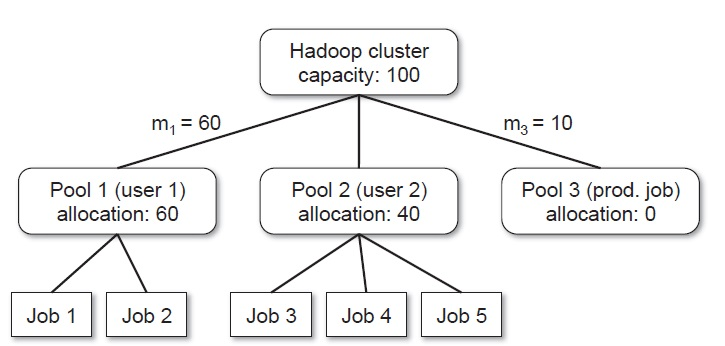
\includegraphics[scale=0.8]{pools.jpg}
\end{center}
 \textit{Diagrama de asignaci\'on de slots de FAIR'}.

\vspace{2mm}

Dado el objetivo de FAIR de asignar la totalidad de recursos de un cluster entre las pools que tienen trabajos, la principal pregunta es c\'omo reasignar slots cuando la demanda fluct\'ua. FAIR utiliza una estrategia mixta entre esperar que terminen tareas y \emph{matar} tareas, o finalizarlas forzadamente. Matar tareas no tiene consecuencias graves en \emph{Hadoop}, simplemente se considera que nunca comenzaron.

\vspace{2mm}

Cuando un trabajo comienza, FAIR comienza a asignarle slots a medida que finalizan otros trabajos. Teniendo en cuenta que las tareas Map-Reduce son generalmente cortas, un trabajo alcanza su cantidad minima de slots r\'apidamente, comparable a la velocidad de un cluster privado.
En caso de haber trabajos con tareas largas, FAIR usa dos \textbf{timeouts} para cada trabajo. Uno para garantizar que pasado el tiempo el trabajo haya conseguido su cantidad minima de slots (en caso de que no, FAIR mata tareas de otras pools y reasigna slots al trabajo), el segundo para garantizar que pasado m\'as tiempo obtenga la cantidad \textbf{justa} de slots (caso contrario, mata m\'as tareas).

\vspace{2mm}

Las tareas a matar pertenecen a trabajos sobrecargados, y se buscan las m\'as recientemente empezadas, de forma de minimizar el tiempo de c\'omputo perdido, siempre y cuando no se lleve a la cantidad de slots de un trabajo a menos de su m\'inimo.

\subsection{Problemas asociados a FAIR y sus soluciones}

Los autores analizaron y abordaron los problemas cl\'asicos que todos los schedulers presentan con Map-Reduce y \emph{Hadoop}: localidad y dependencia.

\subsubsection{Delayed Scheduling}

El primer problema de localidad que notaron los autores fue en los trabajos cortos. Ellos nombran al comportamiento causante de esto \emph{head-of-line scheduling}. En cada momento, hay un trabajo que debe recibir el pr\'oximo slot seg\'un el scheduler: el trabajo con m\'as slots de diferencia por debajo que la cantidad justa (el \emph{head-of-line}). Cualquier nodo esclavo que pida una tarea recibe una de este trabajo. Sin embargo, si este trabajo es pequenio, hay muy pocas posibilidades de que sus bloques de entrada est\'en disponibles en el esclavo. Este problema estaba presente en todos los schedulers de \emph{Hadoop} en ese momento.

\vspace{2mm}

El problema presentado deriva de la falta de elecci\'on del scheduler, seguir un orden de asignaci\'on estricto fuerza que se seleccione un trabajo sin datos locales. La soluci\'on de los autores a este problema tiene por nombre \textbf{Delayed scheduling}. Cuando un nodo solicita una tarea, si el trabajo al principio de la fila no posee una tarea local, se saltea y se busca en los siguientes trabajos. Sin embargo, si un trabajo fue demasiado salteado, se le permite lanzar tareas no locales para prevenir \emph{starvation}. 

\vspace{2mm}

Se tienen dos timers, $T1$ y $T2$. Los trabajos inicialmente s\'olo pueden lanzar tareas locales. Si se cumple $T1$, se le permite lanzar tareas del mismo \emph{rack}. Si se cumple $T2$, se le permite lanzar tareas fuera del \emph{rack}. Si un trabajo inicia una tarea \emph{mas local} que el nivel en el que est\'a, vuelve a un nivel anterior, de forma de que si un trabajo tiene mala suerte al inicio de su vida no se queda lanzando tareas no locales para siempre.

\vspace{2mm}


\subsubsection{Copy-Compute Splitting}

Como se explic\'o anteriormente, las funciones Map generan resultados intermedios, que almacenan en disco, y las funciones Reduce copian estos resultados, y luego deben esperar que todas las Map finalicen para generar la reducci\'on. Esto genera acumulaci\'on de slots de Reduce por parte de trabajos largos que a\'un no pueden ejecutar, generando \emph{starvation} para trabajos cortos y subutilizando recursos.

\vspace{2mm} 

El problema subyacente es que una funci\'on reduce se divide en dos operaciones con requerimientos de recursos distintos. Una copia intensiva de E/S y una reducci\'on intensiva de CPU. En cada momento, un slot se encuentra copiando, usando E/S, o computando, usando CPU, y nunca ambas cosas. Dado que las funciones Reduce se disparan cuando finalizan las Map, se ejecutan en \emph{olas}, causando que todos los slots se encuentren o copiando o computando en un momento dado. Los trabajos se ejecutar\'ian m\'as eficientemente si ambas etapas pudiesen superponerse. Los autores presentan una soluci\'on llamada \emph{copy-compute splitting}, que divide los Reduce en dos tareas: \textbf{copiar y computar}.

\vspace{2mm} 

Las tareas \textbf{copiar} hacen \emph{fetch} y \emph{merge} de la salida de las funciones Map, operaciones de entrada y salida de red. Las tereas \emph{computar} aplican la funci\'on reduce del usuario a la salida de Map. Esto fue implementado agregando una etapa de control de admisi\'on a los procesos Reduce originales de \emph{Hadoop}. Cuando una funci\'on reduce termina de copiar y mergear, pide permiso a su esclavo para iniciar la fase computar. El esclavo limita la cantidad de funciones reduccice computando en un momento dado. Esto permite a los nodos ejecutar m\'as funciones reduce que los slots de c\'omputo que posee. Tambi\'en limita el n\'umero de funciones reduce en fase de copiar de un nodo a la cantidad de slots de c\'omputo que posee, permitiendo a otros trabajos usar los restantes slots.

\vspace{2mm} 

\subsubsection{Tiempo de respuesta Batch}

Contraintuitivamente, un scheduler de algoritmo FIFO puede ser m\'as efectivo en el tiempo de respuesta de las tareas \emph{batch}, incluso con \emph{copy-compute splitting} activado. Esto se debe a que con \emph{fair sharing}, suponiendo dos tareas iniciales, ambas se dividen los recursos y ejecutan al mismo tiempo tareas Map, compiten por la E/S, y luego ambos ejecutan tareas Reduce. En cambio, con un algoritmo FIFO, la primer tarea recibe los slots de Map, y cuando \'esta termina y pasa a la etapa Reduce, la segunda tarea comienza con las tareas Map, generando un pipeline de c\'omputo, acelerando la ejecuci\'on total. Los autores encontraron que el tiempo de respuesta \emph{batch} para el algoritmo FIFO es igual o superior a cualquier otro.

\subsubsection{Utilizaci\'on de espacio en disco}

Una consecuencia final de la dependencia de datos, es la alta utilizaci\'on de espacio en disco para el almacenamiento de los resultados intermedios de las funciones Map. Los autores encontraron que un scheduler FIFO vuelve a sacar ventaja, ya que usa el m\'inimo espacio requerido por las tareas por correrlas secuencialmente. \emph{Fair sharing} puede usar $N$ veces m\'as espacio, siendo $N$ la cantidad de usuarios del cluster.

\subsection{Testing y evaluac\'on}

Los autores evaluaron el scheduler previamente presentado mediante un \emph{Microbenchmark} que muestra los efectos particulares de los componentes, y un \emph{Macrobenchmark} que simula la carga de trabajo multi-usuario de \emph{Facebook}. Los experimentos fueron realizados en tres cl\'usters: \emph{Amazon Elastic Compute Cloud}, un \emph{hosting enviroment} virtual comercial, un cluster de 100 nodos y uno de 450. Para generar la carga de trabajos se utiliz\'o \emph{Loadgen}, un trabajo configurable que tiene dos porcentajes, $keepMap$, que es el porcentaje de los datos de input que devuelven las tareas map, y $keepReduce$, el porcentaje de ouput de Map que devuelven las tareas Reduce.

\subsubsection{Macrobenchmark}

Se evalu\'o un benchmark multi-usuario en el cluster de \emph{Amazon}, con trabajos basados en la carga de \emph{Facebook}. Se us\'o $Loadgen$ con porcentajes random y tiempo de CPU random por trabajo. Consisti\'o en 50 trabajos, de 9 tamanios diferentes, y una cantidad de trabajos por cada tamanio proporcional al de \emph{Facebook} para cada tamanio. Los benchmarks corrieron aproximadamente 30-40 minutos y se compar\'o el scheduler FIFO y el FAIR, con y sin \emph{compy-compute splitting}, y FAIR con \emph{compy-compute splitting} y \emph{delay scheduling}.

\vspace{2mm}

Los resultados mostraron que \emph{fair sharing} puede reducir los tiempos de respuesta a la mitad con respecto a FIFO en trabajos cortos, pero los trabajos largos tardan ligeramente m\'as tiempo. FAIR con \emph{c-c splitting} mejora la velocidad en un $4.6x$ para trabajos cortos, y $1.8-2x$ para los promedio. FIFO \emph{c-c splitting} mejora el tiempo pero sus mejoras son menos notables a las de FAIR.

\vspace{2mm}

El agregado de \emph{delay scheduling} no cambia el tiempo de respuesta de FAIR con \emph{c-c splitting}. Sin embargo, incrementa la localidad a $99-100\%$, cuando originalmente era $15-95\%$, lo cual incrementa el throughput en clusters con menor banda ancha. En resumen, para trabajos cortos y medios, las mejoras promedio fueron de $2.5-5x$, con m\'aximos de $14x$.

\subsubsection{Microbenchmarks}

Se realizaron los siguientes experimentos:

\begin{itemize}

\item \emph{Delay scheduling} y localidad: Se testearon los efectos de esta t\'ecnica en la localidad de trabajos cortos, generando tareas random y usando el cluster m\'as chico. Cada trabajo es map-only, simulando tareas de filtro de datos. Se corrieron trabajos de 3, 10 y 100 tareas, por 20 minutos en total. FIFO dio los mismos resultados que FAIR, tanto con \emph{delay scheduling} como sin.

\emph{Delay scheduling} increment\'o el throughput por $1.2x$ para los trabajos de 3-map, $1.7x$ para los 10-map, y $1.3x$ para los 100-map, e increment\'o la localidad de datos en nodo hasta un $75\%$ y de rack hasta un $94\%$. La mejora de throughput es mayor para los trabajos de 10 map que para los de 100, ya que los trabajos de 100 maps ya tienen buena localidad de por si sin la t\'ecnica.

\item \emph{Delay scheduling} y el tiempo de respuesta: Se testearon los efectos de esta t\'ecnica en el tiempo de respuesta de trabajos 16-map y 1-reduce cada uno. Se corri\'o cada trabajo ocho veces. Corriendo solo, cada trabajo tard\'o entre $32-37s$, y con \emph{delay scheduling}, $32-38s$. No hubo diferencia en tiempo de respuesta, pero la localidad aument\'o de $25\%$ a $100\%$.

\item Carga de E/S: Se cre\'o un archivo de 2GB con triple r\'eplica. Se simularon 20 trabajadores, que iniciaban trabajos durante 20 minutos. 10 se dedicaron a inciar trabajos E/S intensivos, y los otros 10 CPU intensivos. Luego de pasar 10 minutos se cuenta el total de trabajos terminados. Para \emph{delay scheduling} sin modificaciones se obtuvo el peor throughput y tiempo de respuesta. Desactivandolo se obtuvieron mejores resultados, simplemente porque las tareas CPU, que no utilizan E/S, pueden iniciar m\'as r\'apido. Sin embargo, utilizando \emph{delay scheduling} con \emph{IO-rate biasing}, es decir, retardando s\'olo las tareas de los trabajadores E/S llev\'o a la mejor performance posible, con una mejora de $8\%$ para E/S y $10\%$ para CPU.

\item \emph{Copy-Compute splitting} para un solo trabajo: los autores notaron una mejora del $9\%$ en un solo trabajo para un solo usuario, debido a que hay poca mejora para t\'ecnica a menos que el ancho de banda sea limitado. Esperan mejores resultados para clusers de mayor tamanio.

\end{itemize}

\subsection{Discusi\'on y conclusiones}

A pesar de que Map-Reduce nace como un modelo popular para la ejecuci\'on de tareas \emph{batch}, muchas organizaciones comenzaron a compartir sus clusters de \emph{Hadoop} Map-Reduce entre diversos usuarios, corriendo tareas \emph{batch}, pero adem\'as tareas cortas e interactivas. El trabajo nace de la necesidad de un scheduler eficiente para este nuevo caso de uso, ya que el scheduler base FIFO presentaba diversos problemas. Los autores desarrollaron y presentan FAIR, un scheduler que provee aislamiento, garantiza una cantidad de slots m\'inica para cada trabajo y logra \emph{statistical multiplexing}.

\vspace{2mm}

El trabajo de los autores se relaciona con la discusi\'on y \emph{trade-off} entre tener un cluster privado para cada usuario, que brinda el mejor aislamiento, pero provoca subutilizaci\'on y es costoso, y tener un \'unico cluster FIFO, que provee la mejor utilizaci\'on de los recursos pero aislamiento pobre. El objetivo de los autores fue buscar y encontrar un punto medio entre ambas cosas, compartir un cluster eficientemente, brindar a cada usuario tiempos de respuesta similares a clusteres privados y consolidar los datos, teniendo grandes vol\'umenes de datos para el uso de aplicaciones que no podr\'ian correrse en clusteres pequenios con los datos particionados. Los problemas m\'as t\'ipicos presentados en clusters Map-Reduce, la localidad y la interdependencia de datos, se presentan en la mayor\'ia de los servidores que usan grafos ac\'iclicos para modelar y gestionar procesos, por lo que las t\'ecnicas presentadas por los autores, \emph{delay scheduling} y \emph{copy-compute splitting} pueden usarse en cualquier sistema basado en flujo de datos.

\vspace{2mm}

Los autores, luego de su trabajo de investigaci\'on se toman la libertad de brindar algunas recomendaciones acerca de la gesti\'on de scheduling de clusters multi-usuario. En resumen:

\begin{itemize}

\item \textbf{Tareas cortas:} mantener preferencia por tareas cortas y livianas. De esta forma, los trabajos pueden iniciar m\'as r\'apidamente. Limitar los recursos de cada tarea incrementa las oportunidades de scheduling.

\item \textbf{Pausar tareas largas:} Si son necesarias tareas largas, permitir pausarlas. Por ejemplo, pausar tareas de copia para controlar la carga en los esclavos.

\item \textbf{Tradeoff:} Si se requiere aislamiento, se debe sacrificar throughput, como lo ilustra \emph{Delay Scheduling}.

\item \textbf{Localidad de c\'odigo:} Es beneficioso correr m\'ultiples tareas de un trabajo en el mismo nodo, ya que se amortiza el costo de copiar el c\'odigo del trabajo al nodo.

\end{itemize}
